\section{Introduction}
\label{sec:intro}

Proxies are a powerful to for tasks such as browsing privately and evading censorship. The number of available proxy services on the internet is limited, in part due to lack of incentive for servers to operate. This means it is difficult for users to take advantage of more demanding techniques which require a number of proxies rather than a single one. We offer a solution to this problem by incentivizing proxy servers to join the network through use of Bitcoin micropayments. 

\subsection{Proxies}

One technology associated with proxies is proxy rotation, where a user rotates over a number of different proxies rather than just using one. This allows a user to appear to be many different machines rather than a single computer, hiding traffic from the user's session. This is currently used by web crawlers in order to avoid being blocked by a website by appearing to come from many different IP addresses. With some extension this technique can be applied to general proxy usage. There already exist some proxy services which use a similar model of owning many proxies and rotating a user's traffic through them, but this has the disadvantage of still being centralized on the business entity controlling the proxies.

\subsection{Background on Bitcoin}
\begin{figure*}
  \centering
  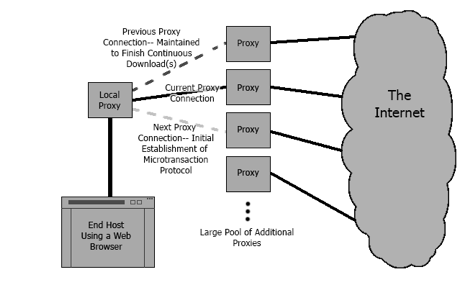
\includegraphics[width=1.05\textwidth]{proxydiagram.png}
  \caption{Diagram of proxy rotation}
  \label{fig:proxy-diagram}
\end{figure*}

Bitcoin\cite{nakamoto2008bitcoin} is a P2P digital currency which has exploded in popularity in the past few years. One of the appeals of Bitcoin is that online transactions do not require third party payment processors. Instead transactions can be included in a global history, called the block chain, in minutes. Additionally, transactions are not strongly tied to a person's identity, as is the case of credit card transactions, but rather tied to a pseudonymous address. Most transactions simply transfer Bitcoins from one address to another, but more complicated types of contracts can be built out of these transactions. We explore how one type of contract, micropayment channels, can be used to facilitate a proxy network. A micropayment channel allows an individual to make small incremental payments to another individual without actually posting a transaction to the block chain. For this case, we have applied micropayment channels so a client will increment their payment to a server when the server provides a service to them. When the channel is closed, a single transaction is posted, resolving many small transactions without publishing each of them on the block chain. Micropayments enable pay as you go type services where payment is immediate and does not suffer from transaction fees.

Although Bitcoin micropayments were first added to the Bitcoin Wiki by core Bitcoin developer Mike Hearn in December 2011,  actual deployment of micropayment based services has been very slow. No observable development happened until June 27, 2013 when BitcoinJ, a prominent java library for Bitcoin, added support for micropayments. Since then some services have been built using micropayments, but these are all specialized services, and these are still very few in number.
